%!TEX root = ../main.tex

\section{Численное исследование}

\subsection{Улучшенная оценка устойчивости}

В предыдущем разделе из анализа уравнения \eqref{eq:spectral} было получено условие \eqref{cond:spectral_0}, необходимое для устойчивости разностной схемы \eqref{sch:transition}, \eqref{sch:borders} при $\phi \approx 0$. Предположение о его полезности основано на том, что типичным поведением модели будет некоторый процесс перехода $\phi$ от $1$ к $0$ (<<разрушение>>) за конечное время, а затем бесконечно долгое пребывание в состоянии $\phi \approx 0$.

Однако проделанного анализа уравнения \eqref{eq:spectral} в точке $\phi = 0$ недостаточно. В самом деле, было использовано, что $\epsilon''(0) = 0$ (см. выражение \eqref{eq:epsilon_phi_phi}), но не учтено, что $\epsilon''(\phi)$ при малых $\delta$ вблизи $0$ растет очень быстро и достигает больших значений (рис.~\ref{fig:eps_phi_phi}). Получается, что модель, устойчивая в точке $0$, может работать неадекватно в малой ее окрестности. Это нас, конечно, не устраивает -- улучшим оценку устойчивости.

\begin{figure}[!tp]
    \centering
    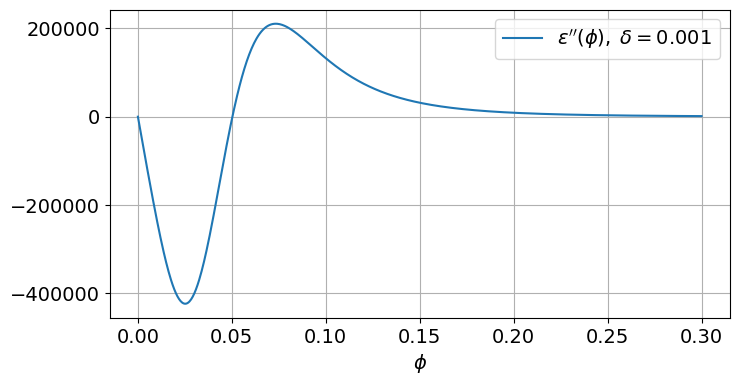
\includegraphics[width=\textwidth]{figures/eps_phi_phi.png}
    \vspace{-0.7cm}
    \caption{Поведение функции $\epsilon''(\phi)$ около $0$.}
    \label{fig:eps_phi_phi}
\end{figure}

Нужно оценить экстремумы функции $\epsilon''(\phi)$ вблизи $0$. Для начала найдем нули $\epsilon'''(\phi)$. Имеем:
$$f'''(\phi) = 24 - 72 \phi; \quad \epsilon'''_{fff} = \cfrac{-6 \epsilon_0}{(f(\phi) + \delta)^4} \tsemicolon$$
\begin{equation}
    \epsilon''' = \epsilon'''_{fff} \cdot (f')^3 + 3 \epsilon''_{ff} \cdot f' \cdot f'' + \epsilon'_f \cdot f''' = \epsilon_0 \cfrac{-6 (f')^3 + 6 (f + \delta) f' f'' - (f + \delta)^2 f'''}{(f + \delta)^4} \tpoint
    \label{eq:epsilon_phi_phi_phi}
\end{equation}
Приравняв $\epsilon'''$ к $0$, получим:
$$-6 (f')^3 + 6 (f + \delta) f' f'' - (f + \delta)^2 f''' = 0 \tcomma$$
или
\begin{multline*}
    -6(12 \phi^2 (1 - \phi))^3 + 6(4 \phi^3 - 3\phi^4 + \delta) \cdot 12 \phi^2 (1 - \phi) \cdot 12 \phi (2 - 3\phi) - \\ - (4 \phi^3 - 3 \phi^4 + \delta)^2 \cdot 24 (1 - 3 \phi) = 0 \tpoint
\end{multline*}
Разделим последнее уравнение на $24\phi^6$, получим:
$$-3 \cdot 12^2 (1 - \phi)^3 + 36 \left(4 - 3\phi + \cfrac{\delta}{\phi^3} \right)(1 - \phi)(2 - 3\phi) - \left(4 - 3 \phi + \cfrac{\delta}{\phi^3} \right)^2 (1 - 3 \phi) = 0 \tpoint$$
Пусть $\delta_n \to +0$ и корень $\phi_n \to +0$, причем $\delta_n/\phi_n^3$ ограничено. Тогда:
$$-3 \cdot 12^2 \cdot 1^3 + 36 \left(4 + \cfrac{\delta_n}{\phi_n^3} \right) \cdot 1 \cdot 2 - \left(4 + \cfrac{\delta_n}{\phi_n^3} \right)^2 \cdot 1 \to 0 \tcomma$$
$$\left(4 + \cfrac{\delta_n}{\phi_n^3} \right)^2 - 72 \left(4 + \cfrac{\delta_n}{\phi_n^3} \right) + 3 \cdot 12^2 \to 0 \tpoint$$
Значит, последовательность $4 + \delta_n/\phi_n^3$ имеет не более двух частичных пределов $\xi_+$ и $\xi_-$ -- корней уравнения $\xi^2 - 72 \xi + 432 = 0$. Первому корню $\xi_+ = 36 + 12 \sqrt{6}$ соответствует
$$\phi = \cfrac{1}{\sqrt[3]{32 + 12 \sqrt{6}}} \sqrt[3]{\delta_n} \approx \cfrac{1}{3.945} \sqrt[3]{\delta_n} \tcomma$$
второму корню $\xi_- = 36 - 12 \sqrt{6}$ соответствует
$$\phi = \cfrac{1}{\sqrt[3]{32 - 12 \sqrt{6}}} \sqrt[3]{\delta_n} \approx \cfrac{1}{1.376} \sqrt[3]{\delta_n} \tpoint$$

Из проделанного рассуждения следует, что при $\delta \to +0$ функция $\epsilon'''(\phi)$ имеет в окрестности $0$ два корня
\begin{equation}
    \phi_{\pm} = \cfrac{1}{\sqrt[3]{32 \pm 12 \sqrt{6}}} \sqrt[3]{\delta} [1 + o(1)] \tpoint
    \label{eq:epsilon_phi_phi_phi_roots}
\end{equation}

Оценим $\epsilon''(\phi)$ в точках $\phi_{\pm}$ при $\delta \to +0$. Пусть $\phi = (1/c) \sqrt[3]{\delta}, \; c \in \Real$. Тогда:
\begin{multline*}
    \cfrac{\epsilon''}{\epsilon_0} = \cfrac{2(f')^2 - (f + \delta)f''}{(f + \delta)^3} = \cfrac{2 \cdot 12^2 \phi^4 (1 - \phi)^2 - (4 \phi^3 - 3 \phi^4 + \delta) \cdot 12 \phi (2 - 3 \phi)}{(4 \phi^3 - 3 \phi^4 + \delta)^3} = \\ = \cfrac{2 \cdot 12^2 - 8 \cdot 12 - 24 (\delta/\phi^3)}{4^3 + 3 \cdot 4^3 (\delta/\phi^3) + 3 \cdot 4 (\delta/\phi^3)^2 + (\delta/\phi^3)^3} \cdot \cfrac{1}{\phi^5}[1 + o(1)] = c^5 \delta^{-5/3} \cfrac{24(8 - c^3)}{(4 + c^3)^3}[1 + o(1)] \tpoint
\end{multline*}
Отсюда:
\begin{equation}
    \epsilon''(\phi_+) \approx -4.378 \epsilon_0 \delta^{-5/3}; \quad \epsilon''(\phi_-) \approx 2.216 \epsilon_0 \delta^{-5/3} \tpoint
    \label{est:epsilon_phi_phi_bounds}
\end{equation}
Оценки экстремумов $\epsilon''(\phi)$ вблизи $0$ показаны на рис. \ref{fig:eps_phi_phi_multiplied}.

\begin{figure}[!tp]
    \centering
    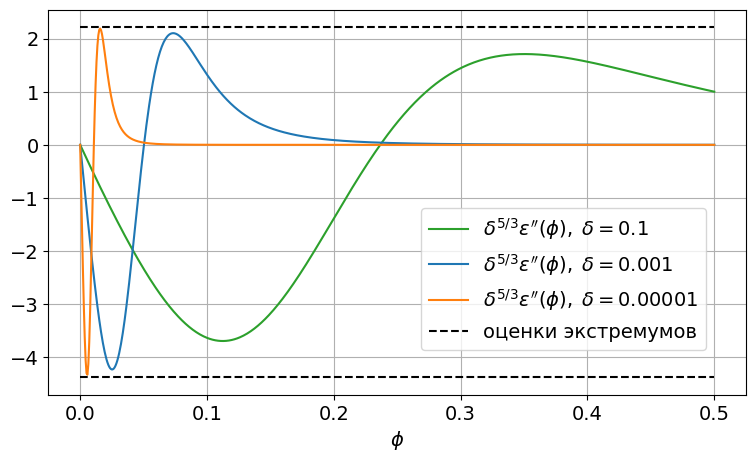
\includegraphics[width=\textwidth]{figures/eps_phi_phi_multiplied.png}
    \caption{Сравнение функций $\delta^{5/3} \epsilon''(\phi)$ при различных значениях $\delta$.}
    \label{fig:eps_phi_phi_multiplied}
\end{figure}

Получим новую оценку устойчивости, рассмотрев уравнение \eqref{eq:spectral} в точке $\phi = \phi_+$. $\epsilon''(\phi_+) \approx -4.4 \epsilon_0 \delta^{-5/3}$. Сумма в скобках отрицательна ($\delta$ мало, $\epsilon''(\phi_+)$ велико по модулю и отрицательно), поэтому $f''(\phi_0) > 0$ можно считать равным $0$: оценку это только усилит. Преобразовав уравнение \eqref{eq:spectral}, получим:
$$\lambda(\theta) = 1 + m \tau \left( -\cfrac{2.2 K_\Phi^2 \epsilon_0}{\delta^{5/3}} - \cfrac{2 \Gamma}{h^2} \sin^2 \cfrac{\theta}{2} \right) \tpoint$$
Условие $|\lambda(\theta)| \leqslant 1$ справедливо для любого $\theta$, если и только если
\begin{equation}
    \tau \leqslant \left( \cfrac{1.1 m K_\Phi^2 \epsilon_0}{\delta^{5/3}} + \cfrac{m \Gamma}{h^2} \right)^{-1} \tpoint
    \label{cond:spectral_better_theoretical}
\end{equation}

Для применения на практике оценку \eqref{cond:spectral_better_theoretical} нужно брать <<с запасом>> (экспериментальное обоснование будет дано позже). Сделаем оценку строже, примерно удвоив знаменатель:
\begin{equation}
    \tau \leqslant \cfrac{1}{2m} \left( \cfrac{K_\Phi^2 \epsilon_0}{\delta^{5/3}} + \cfrac{\Gamma}{h^2} \right)^{-1} \tpoint
    \label{cond:spectral_better}
\end{equation}

Более простая оценка не слабее оценки \eqref{cond:spectral_better} выглядит следующим образом:
\begin{equation}
    \tau \leqslant \cfrac{1}{4m} \min \left(\cfrac{\delta^{5/3}}{K_\Phi^2 \epsilon_0}, \; \cfrac{h^2}{\Gamma} \right) \tpoint
    \label{cond:spectral_better_simpler}
\end{equation}

Полученная оценка \eqref{cond:spectral_better} устойчивости разностной схемы \eqref{sch:transition}, \eqref{sch:borders} содержит все параметры уравнения \eqref{eq:one_dim_simpler}, кроме $l$.